\documentclass[landscape,xcolor={table},10pt]{beamer}

\usepackage{amsmath}
\usepackage{graphicx}
\usepackage[english]{babel}
\usetheme{Antibes}
\usepackage{tikz}
\usepackage{multimedia}
\usepackage{textpos}
\usepackage{hyperref}
\usepackage{url}
\usepackage{siunitx}

\usetheme{default}
\usecolortheme{seahorse}
\usefonttheme[onlymath]{serif}
\setbeamertemplate{caption}[numbered]
\graphicspath{ {images/} }

\pgfdeclareimage[width=\paperwidth]{mybackground}{images/blue_sun.png}
\pgfdeclareimage[width=0.2\paperwidth]{rocket}{images/launch}

\setbeamertemplate{title page}{

        \begin{picture}(0,0)

            \put(-30,-250){%
                \pgfuseimage{mybackground}
            }

            \put(-168,-100){%
                \begin{minipage}[b][45mm][t]{226mm}
                
                	\centering
               
                  {\usebeamerfont{title}\color{black}\inserttitle \par}
                  
                  \color{black}\insertauthor
                  
                  \insertinstitute
                  
                  \insertdate
                  
                
                  
                \end{minipage}
            }

            \end{picture}
            
            \begin{textblock*}{100mm}(-0.75cm,-3.5cm)
            
\includegraphics[width=2cm]{images/nasa}
            \end{textblock*}

            \begin{textblock*}{100mm}(0.90\textwidth,-3.75cm)
            
\includegraphics[width=2cm]{images/inverted_solar_physics_logo}
            \end{textblock*}

    }

\title[...]{
\includegraphics[width=2cm]{images/moses_logo_with_text}  \\Command and Data Handling for \\ MOSES II Flight Operations}
\author[Smart, Remington]{Roy Smart \and Jackson Remington}
\institute{
\includegraphics[width=2cm]{images/msu}}
\date{May 1st, 2015 \\ }

\addtobeamertemplate{frametitle}{}{%
\begin{textblock*}{100mm}(.45\textwidth,-1.7cm)

\includegraphics[width=2cm]{images/nasa} \;

\includegraphics[width=2cm]{images/msu}	\;

\includegraphics[width=2cm]{images/ssel}
\end{textblock*}}

	
\begin{document}

	\begin{frame}[plain]
	        \titlepage
	\end{frame}
	
	\begin{frame}
		
		\frametitle{MOSES Scientific Goals}
		
		\begin{columns}[T] % align columns
		\begin{column}{.48\textwidth}

			\begin{itemize}
				\item Transition region Explosive Events (EEs)
				\item Extreme UltraViolet wavelengths (EUV)
				\begin{itemize}
					\item Each of the three orders $(m=-1,0,+1)$ are dispersed by multilayer diffraction grating
					\item Observes Ne VII (465\AA) and C III (459\AA) spectral lines 
				\end{itemize}				
				\item Atmospheric absorption of EUV requires space-based observations.
				\item Sounding rocket provides $\sim300$-seconds above 160km.
			\end{itemize}
			
		\end{column}%
		\hfill%
		\begin{column}{.48\textwidth}
		
			
			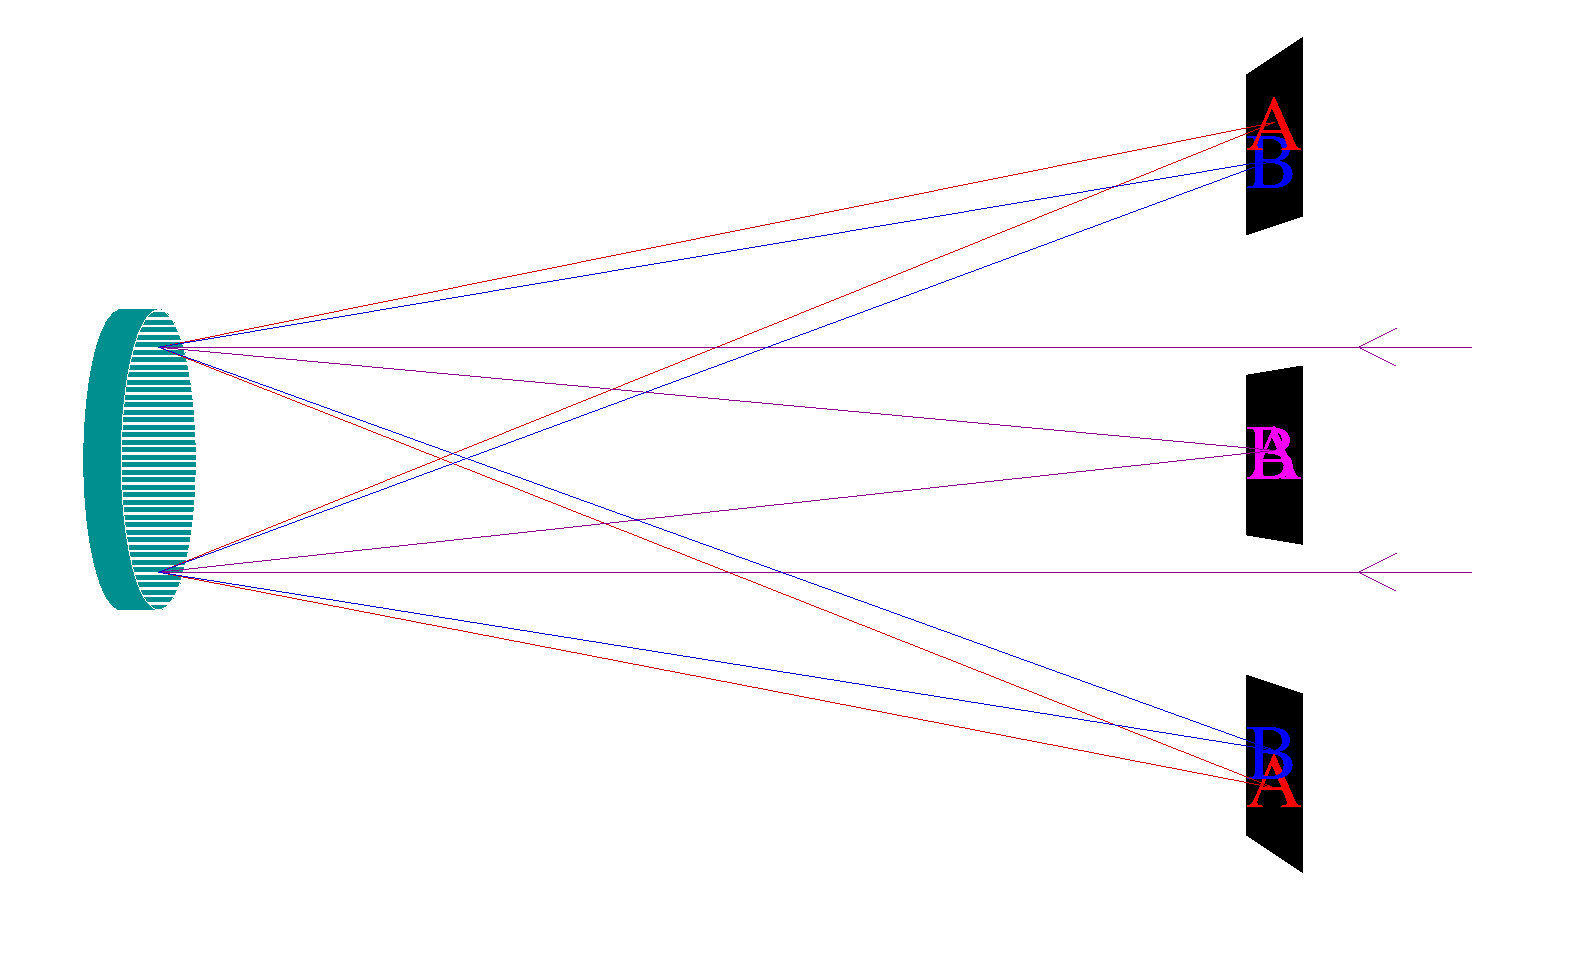
\includegraphics[width=\textwidth]{images/instrument} \\
			\includegraphics[width=\textwidth]{images/inversion}
		
		\end{column}%
		\end{columns}

	\end{frame}
	
	\begin{frame}
		
		\frametitle{First Launch}
		
		\begin{columns}[T] % align columns
		\begin{column}{.15\textwidth}

			\movie[width=3cm,height=7cm,poster,externalviewer]{\pgfuseimage{rocket}}{images/Launch.mp4}
			
		\end{column}%
		\hfill%
		\begin{column}{.83\textwidth}
		
			\begin{itemize}
				\item MOSES first launched on February 8th, 2006 \cite{moses}.
				\begin{itemize}
					\item Utilized a Black Brant IX sounding rocket
					\item Observed the Sun in He II 304 \AA
					\item Identified a Transition Region Explosive Event.
				\end{itemize}
				\item MOSES II
				\begin{itemize}
				%	\item Following the first operation, the MOSES research group planned to try again with updated opticsfor 465 \AA.
					\item Since the previous launch the Hercules flight computer has failed, and a exact replacement is no longer available.
					\item New flight computer was to be developed to act as a drop-in replacement for the old system.
					
				\end{itemize}
			\end{itemize}
			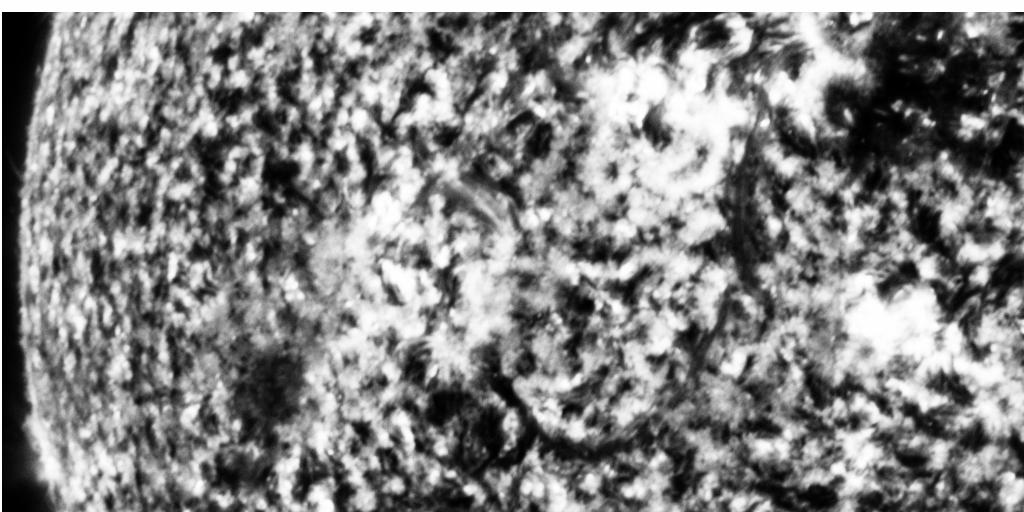
\includegraphics[width=0.7\textwidth]{images/exp2}
		\end{column}%
		\end{columns}
	
	\end{frame}
		
	\begin{frame}
		\frametitle{System Requirements}
		
				\begin{columns}[T] % align columns
				\begin{column}{.49\textwidth}
					\begin{itemize}
						\item Data characteristics
						\begin{itemize}
							\item MOSES captures the sun in three spectral orders $m=-1,0,1$.
							\item Each spectral order is captured by CCDs at $2048 \times 1024$ resolution.
								
						\end{itemize}
					\end{itemize}
					
				\end{column}%
				\hfill%
				\begin{column}{.49\textwidth}
				
					\begin{itemize}
						\item Challenges
						\begin{itemize}
							\item Short flight time, FC must be responsive enough to capture real-time data.
							\item Camera data is presented as 32 Mbit/s unbuffered 16-bit parallel data.
						\end{itemize}
					\end{itemize}
				
				\end{column}%
				\end{columns}
		
		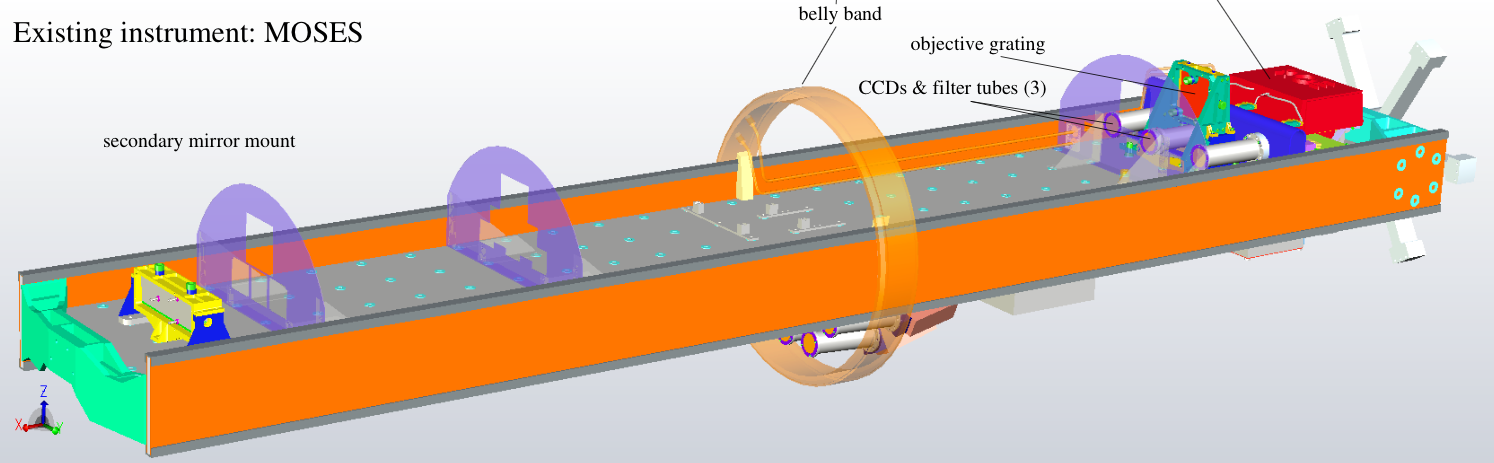
\includegraphics[width=\textwidth]{images/moses}

	\end{frame}
	
	\begin{frame}
		
		\frametitle{Hardware Overview}
		
		\begin{columns}[T] % align columns
		\begin{column}{.68\textwidth}

			\begin{itemize}
				\item Originally planned to replace the Hercules EBX with the TS-7600 embedded system.
				\begin{itemize}
					\item Found that the FPGA implementation was too slow to keep up with the data rate.
				\end{itemize}
				\item VDX104+ Flight Computer (Upper)
				\begin{itemize}
					\item Moderates communications between the ground, cameras, and FPGA.
					\item Executes custom flight software.
				\end{itemize}
				\item Connecttech PCI104 FPGA (Lower)
				\begin{itemize}
					\item Captures parallel data produced by cameras and saves it to a buffer.
					\item Data buffer is copied to the VDX104+ via Direct Memory Access (DMA).
				\end{itemize}
					
			\end{itemize}
		
		\end{column}%
		\hfill%
		\begin{column}{.30\textwidth}

			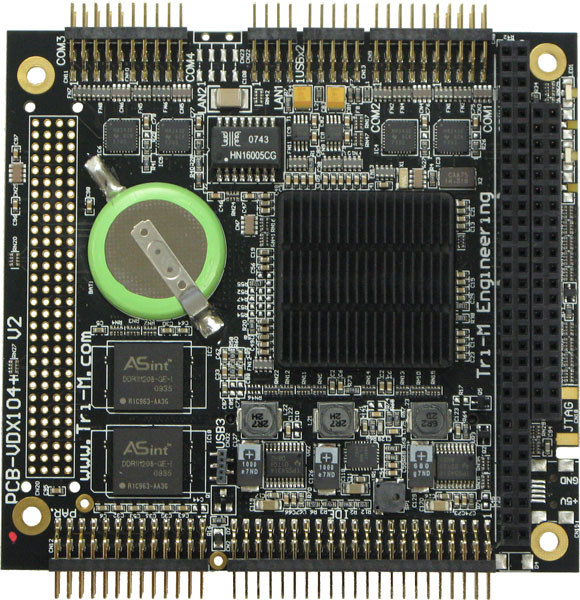
\includegraphics[width=\textwidth]{images/vdx104} \\
			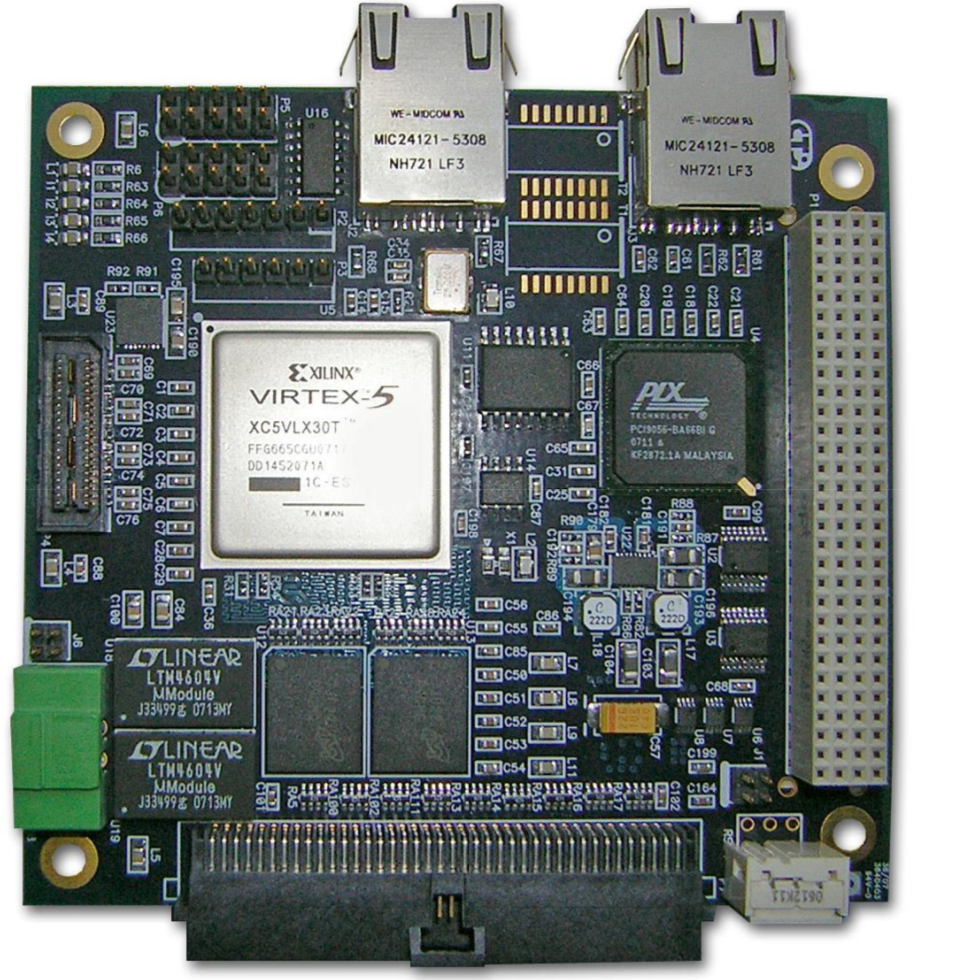
\includegraphics[width=\textwidth]{images/fpga}
					
		\end{column}%
		\end{columns}
			

	\end{frame}
	
	\begin{frame}
		\frametitle{Software Enviroment}
		
				\begin{columns}[T] % align columns
				\begin{column}{.49\textwidth}
					\begin{itemize}
						\item VDX104+ Flight Computer
						\begin{itemize}
							\item Ubuntu 10.04 GNU/Linux operating system with custom kernel.
							\item Flight Software written in the C programming language.
							\item Synclink and ConnectTech software drivers for interfacing with hardware.
						\end{itemize}
					\end{itemize}
				
				\end{column}%
				\hfill%
				\begin{column}{.49\textwidth}
					\begin{itemize}
						\item Ground Station Computer
						\begin{itemize}
							\item Ubuntu 14.04 GNU/Linux OS
							\item Ground station software written in Java.
							\item High-Speed Telemetry software written in the C programming language.
						\end{itemize}
					\end{itemize}
							
				\end{column}%
				\end{columns}
				\begin{center}
					
\includegraphics[height=3cm]{ubuntu-logo}
					
\includegraphics[height=3cm]{c}
					
\includegraphics[height=3cm]{java}
				\end{center}

		
	\end{frame}
	
	\begin{frame}
		
		\frametitle{Flight Software}
		
		\begin{columns}[T] % align columns
		\begin{column}{.60\textwidth}
			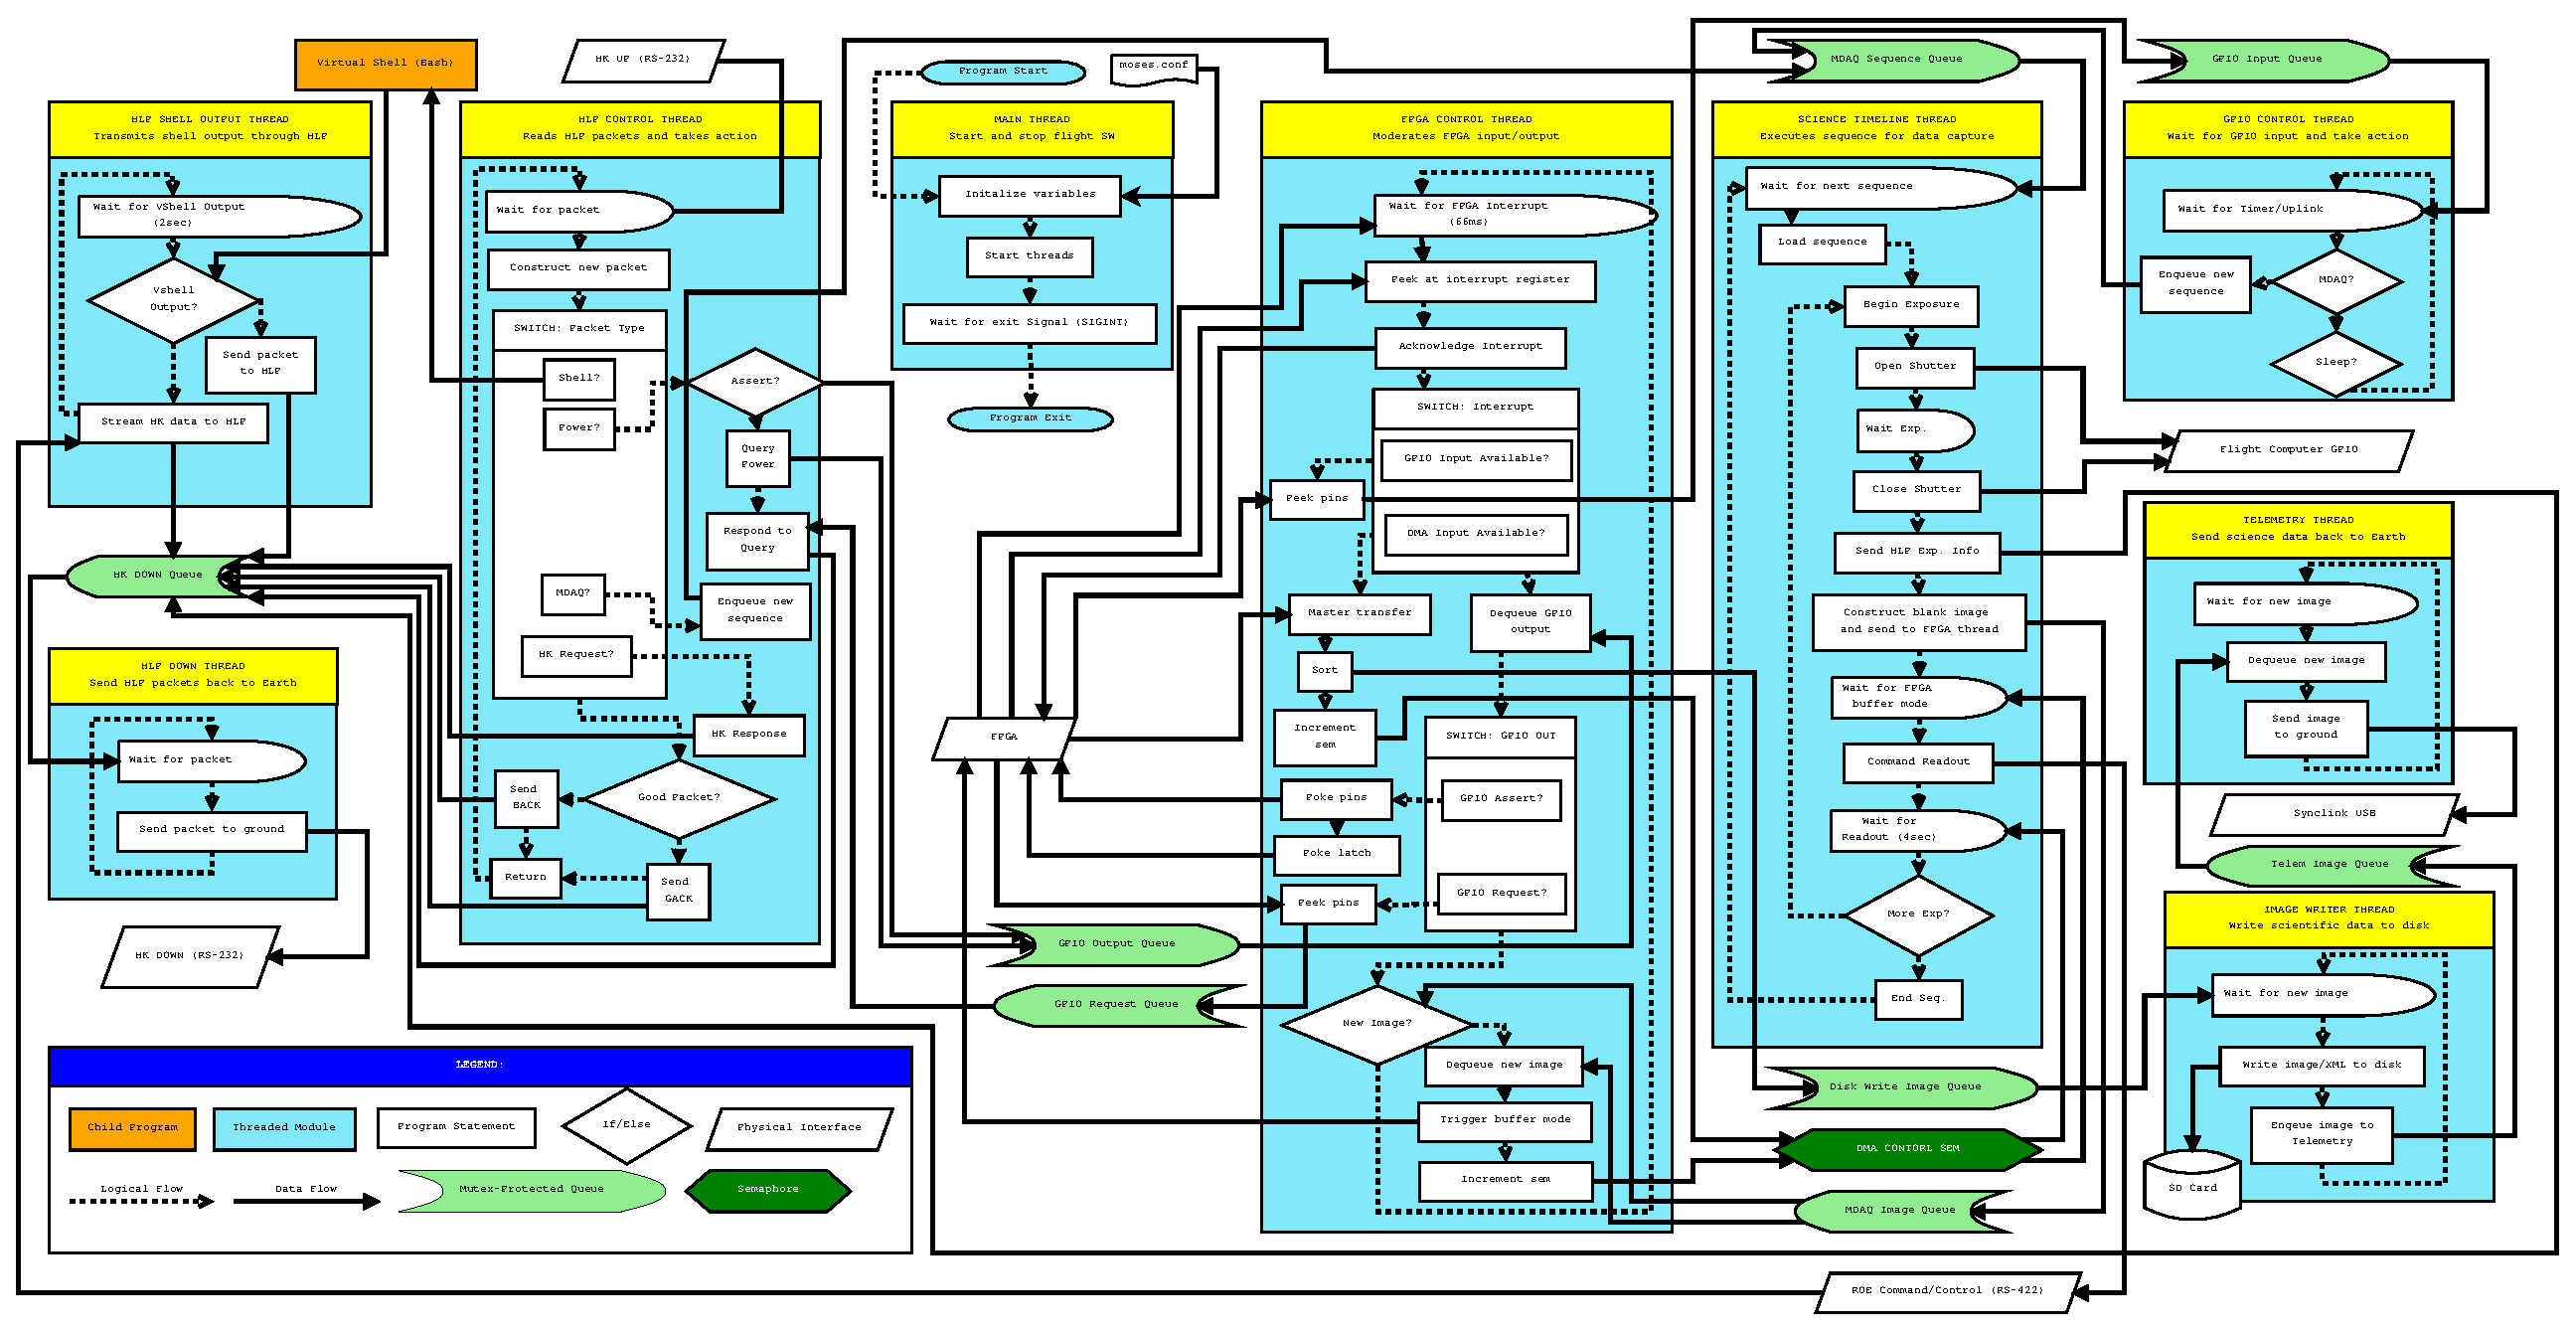
\includegraphics[height=0.85\textheight,clip=true,trim=420 20 220 0]{images/mfsw_block}
		\end{column}%
		\hfill%
		\begin{column}{.39\textwidth}
			\leftmargini=10pt
			\begin{itemize}
				\item Organized into eight concurrent threads for real-time IO.
				\item Main Thread
				\begin{itemize}
					\item Initializes all child threads
				\end{itemize}
				\item Science Timeline Thread
				\begin{itemize}
					\item Executes exposure sequences
					\item Informs FPGA Server of impending images
				\end{itemize}
				\item FPGA Server Thread
				\begin{itemize}
					\item Waits for HW interrupts indicating Timers
					\item Initiates DMA transfer once image is ready
				\end{itemize}
			\end{itemize}
					
		\end{column}%
		\end{columns}
		


	\end{frame}
	
	\begin{frame}
		
		\frametitle{Ground Station}
		
		\begin{columns}[T] % align columns
		\begin{column}{.53\textwidth}

			 \begin{itemize}
				  	\item{Server module: mediates communications between client and payload.}
				  	\item{Client module: transmits Housekeeping Link Protocol (HLP) packets to server via ethernet.}				  	
				  	\item{Debugging communication}
				  	\begin{itemize}
				  		\item{Serial console}
				  		\item{Ethernet}
				  	\end{itemize}
				  	\item{Main in-flight communication}
					\begin{itemize}
				  		\item{Pre-defined Timers}
				  		\item{Uplink push-button switches}
				  	\end{itemize}
				  	
			 \end{itemize}
			
		\end{column}%
		\hfill%
		\begin{column}{.45\textwidth}

			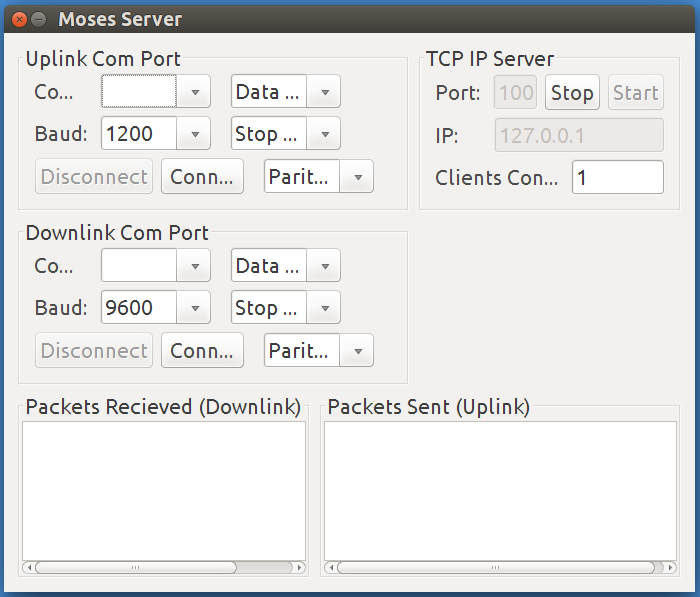
\includegraphics[width=0.7\textwidth]{server_scr} \\
			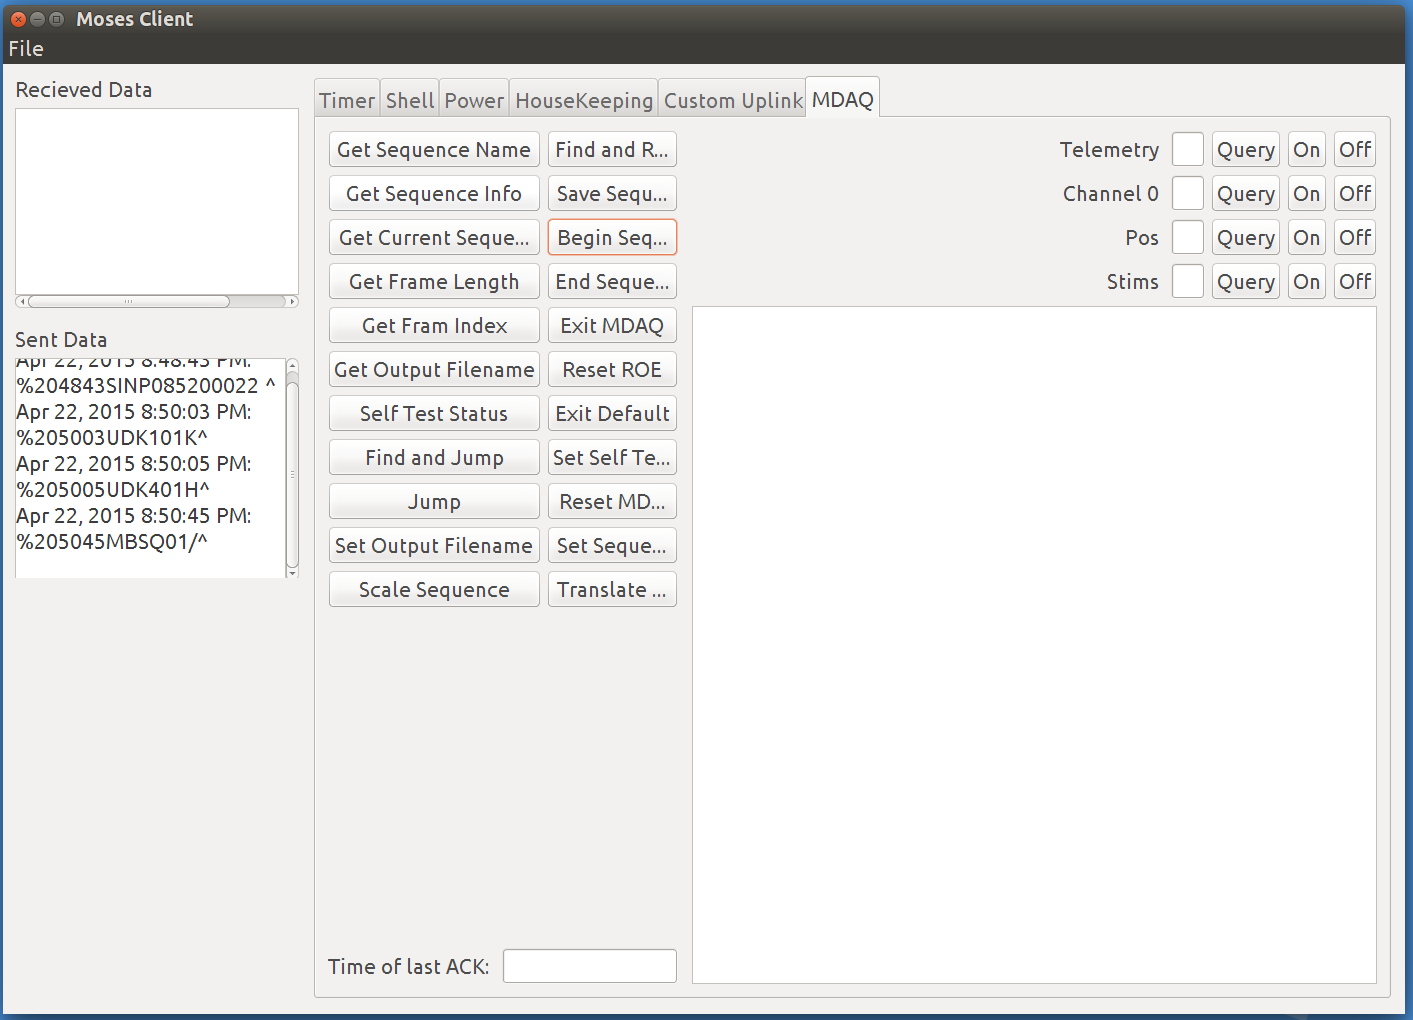
\includegraphics[width=\textwidth]{client_scr}
					
		\end{column}%
		\end{columns}

	\end{frame}
	
	\begin{frame}
		
		\frametitle{Capturing Data}
		
		\begin{columns}[T] % align columns
		\begin{column}{.49\textwidth}
	
			\begin{figure}
				\centering
				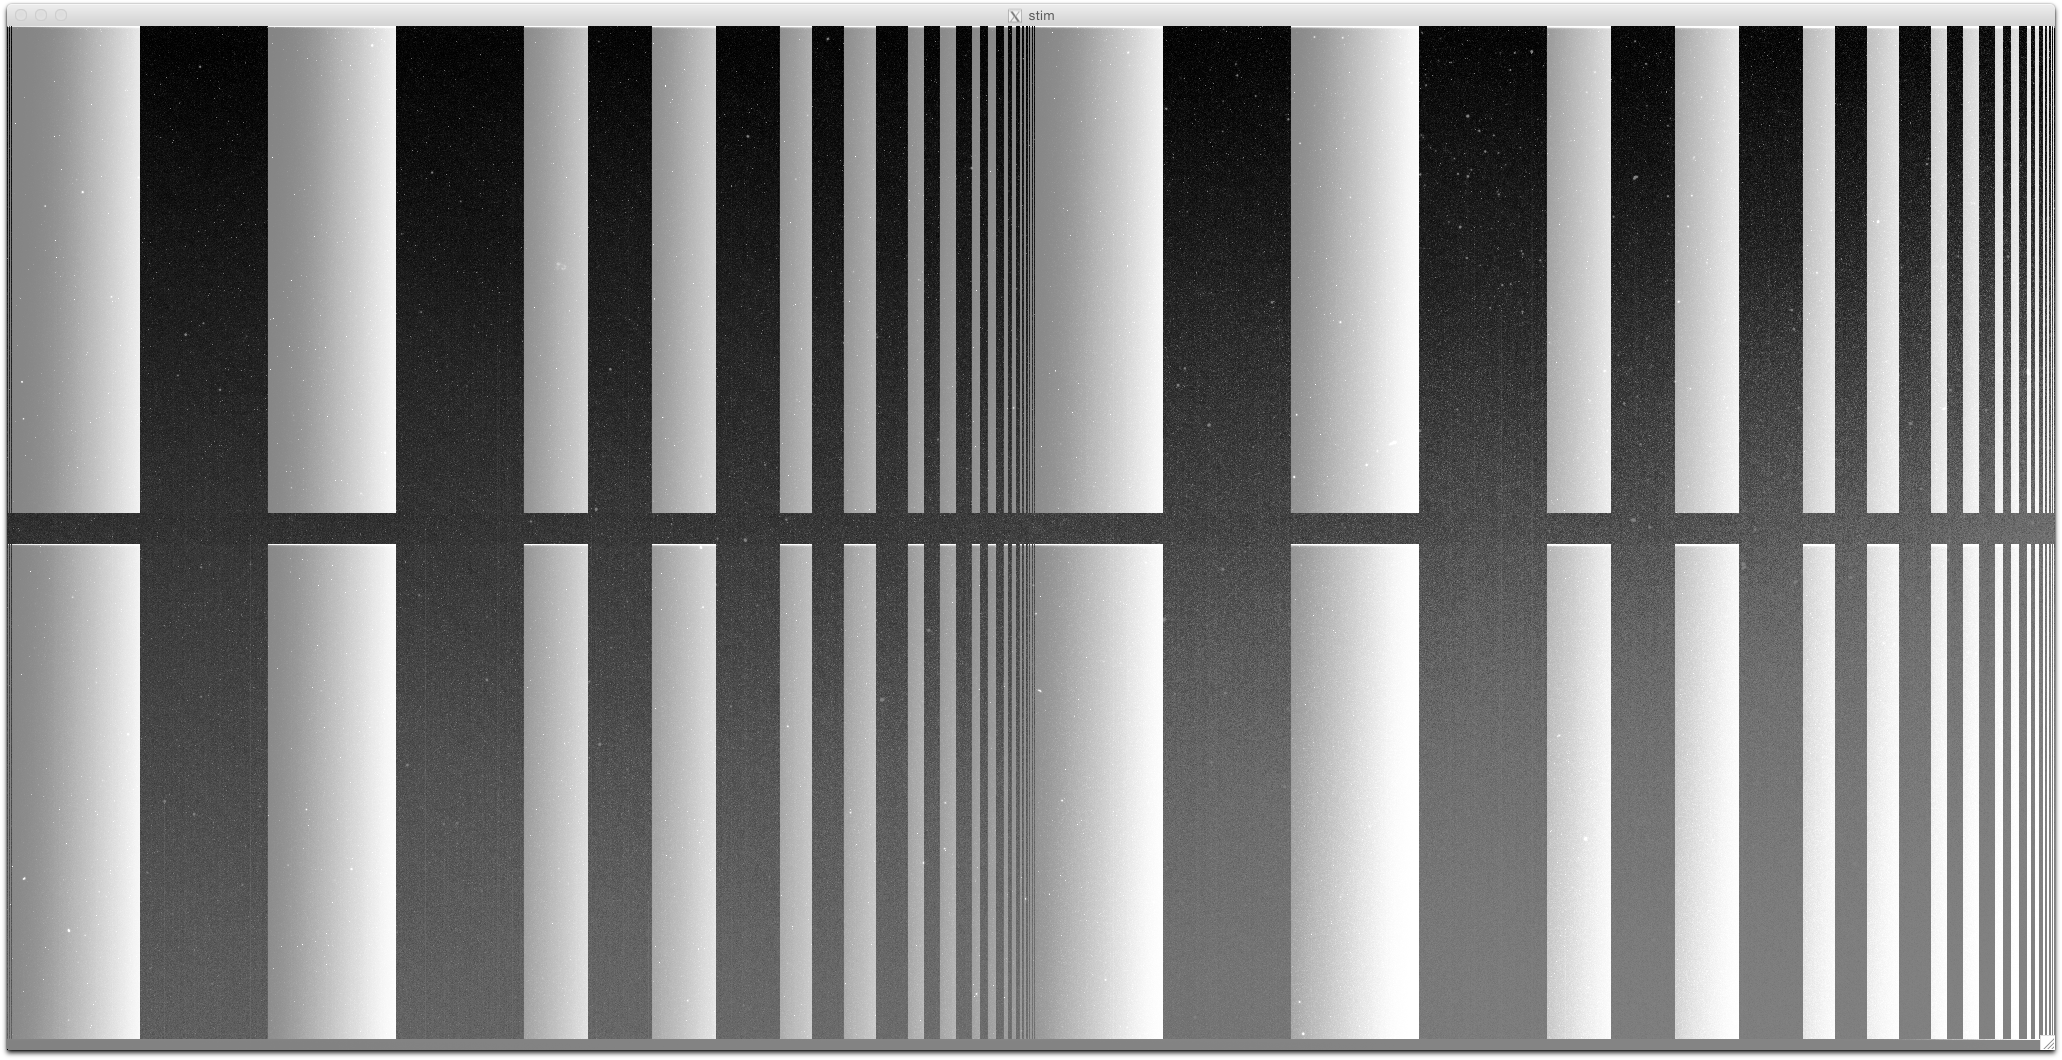
\includegraphics[width=\textwidth]{images/stim_minus} \\
				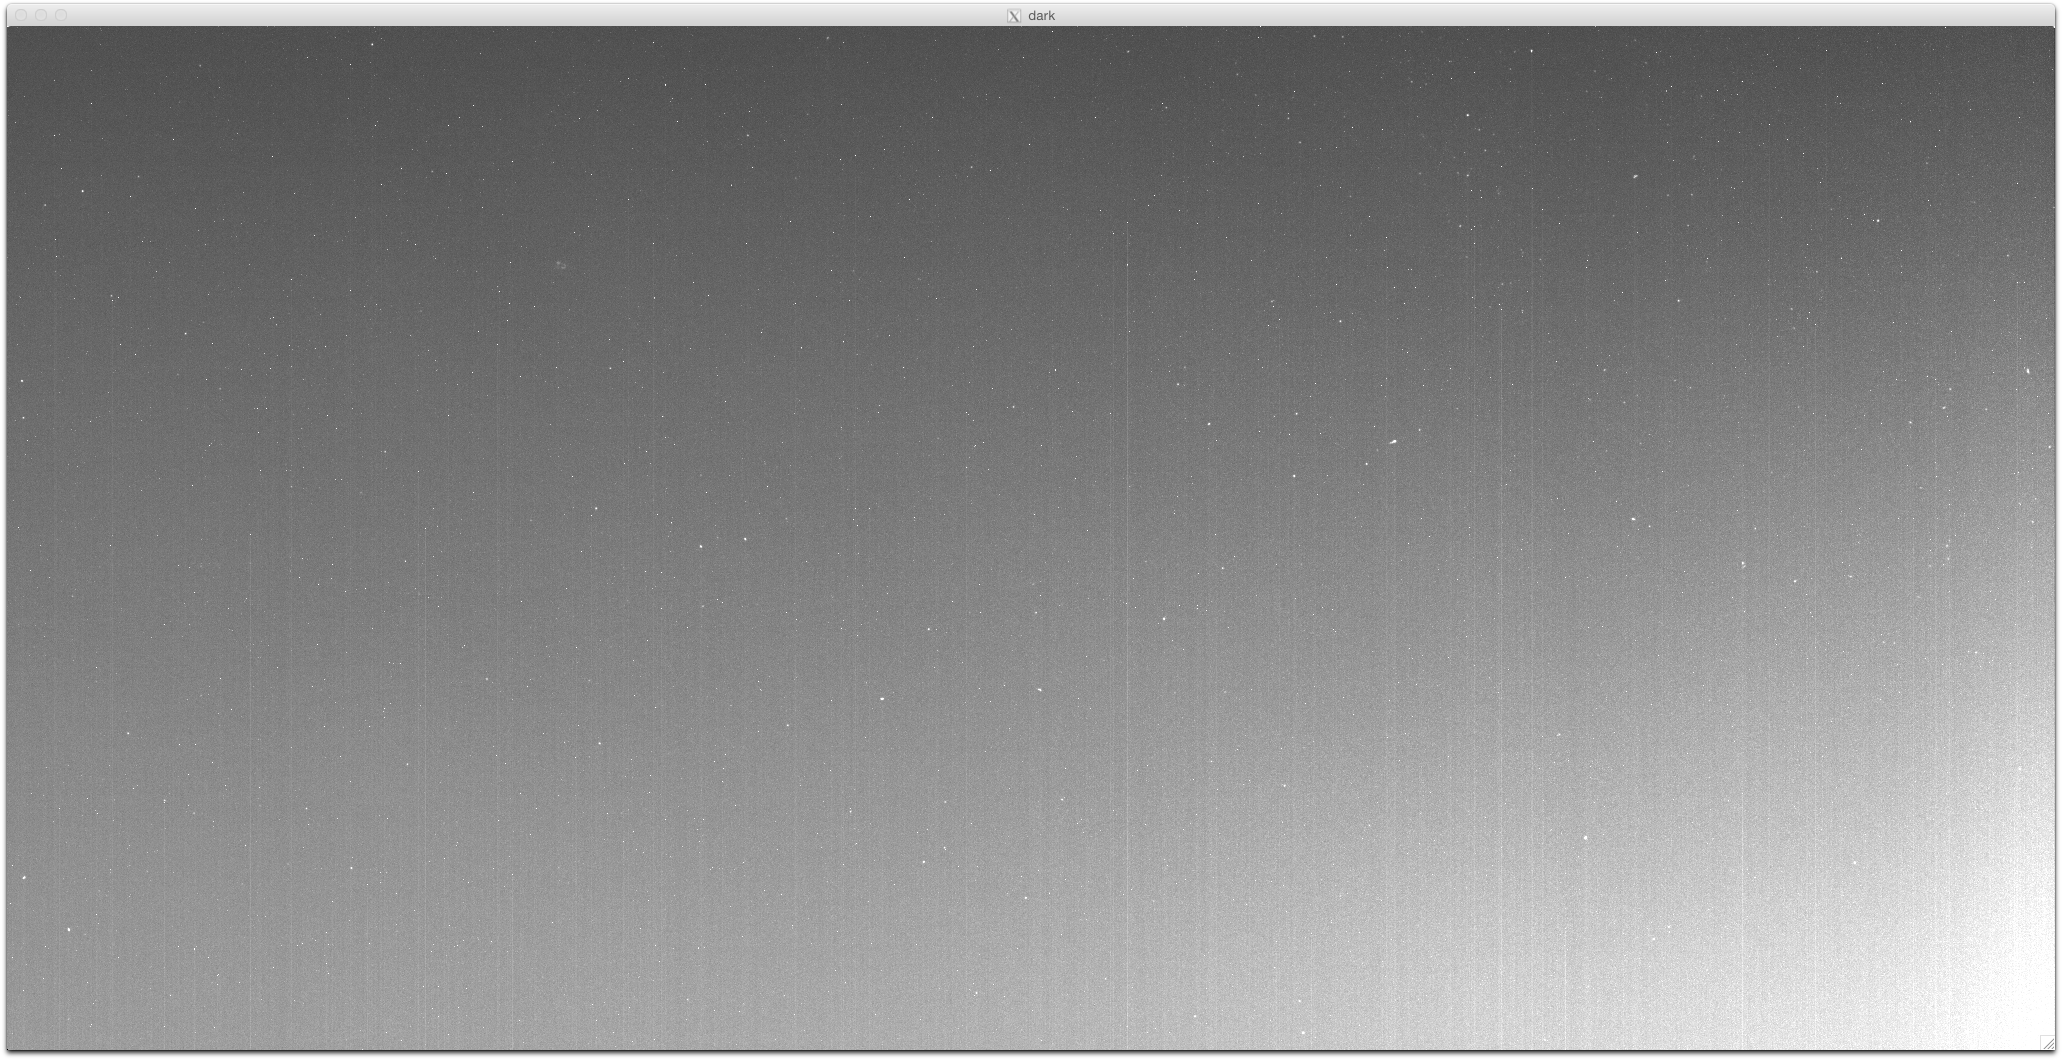
\includegraphics[width=\textwidth]{images/dark_minus}
				\caption{STIMS test image (upper) and a dark exposure (lower).}
			\end{figure}

			
		\end{column}%
		\hfill%
		\begin{column}{.50\textwidth}
		
			\begin{itemize}

		  		\item ReadOut Electronics (ROE)
				\begin{itemize}
			  		\item Each CCD pixel reports 14-bit value proportional to total photons detected over exposure time. 
			  		\item FPGA captures these pixel-maps in three 2-megapixel images
			  	\end{itemize}
		  		\item Flight Software
				\begin{itemize}
			  		\item Opens and closes shutter.
			  		\item Commands ROE to transmit data after exposure complete.
			  		\item Copies data from FPGA to disk.
			  	\end{itemize}
		  	\end{itemize}
		
		\end{column}%
		\end{columns}
		

	\end{frame}
	
	\begin{frame}
		
		\frametitle{Data Retrieval}
		
		\begin{columns}[T] % align columns
		\begin{column}{.49\textwidth}
			\begin{figure}
				\centering
				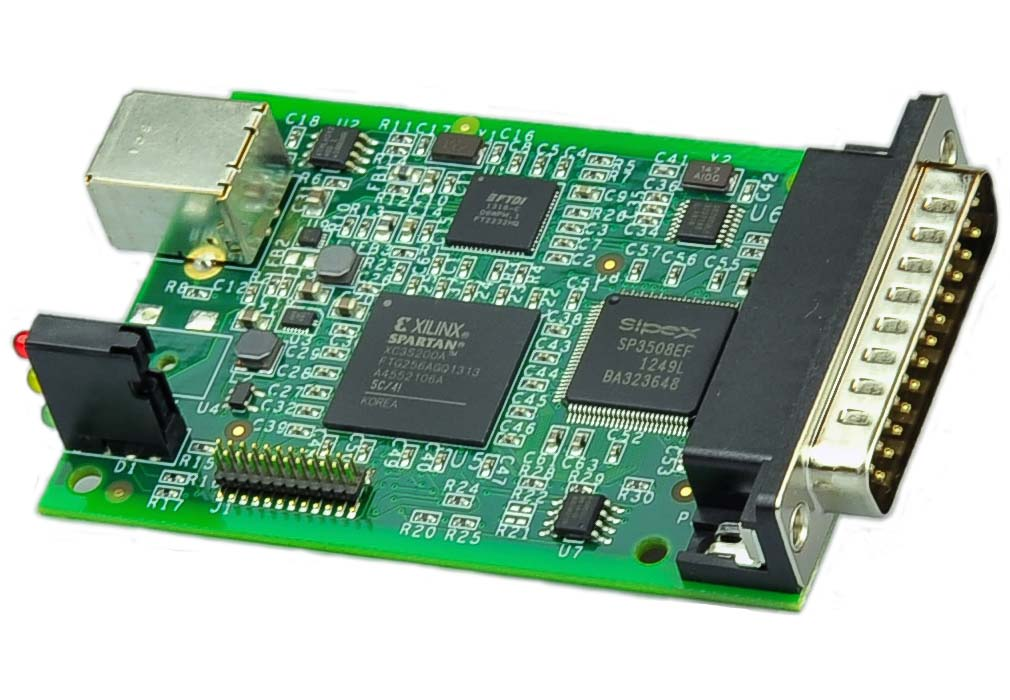
\includegraphics[width=0.6\textwidth]{images/synclink}\\
				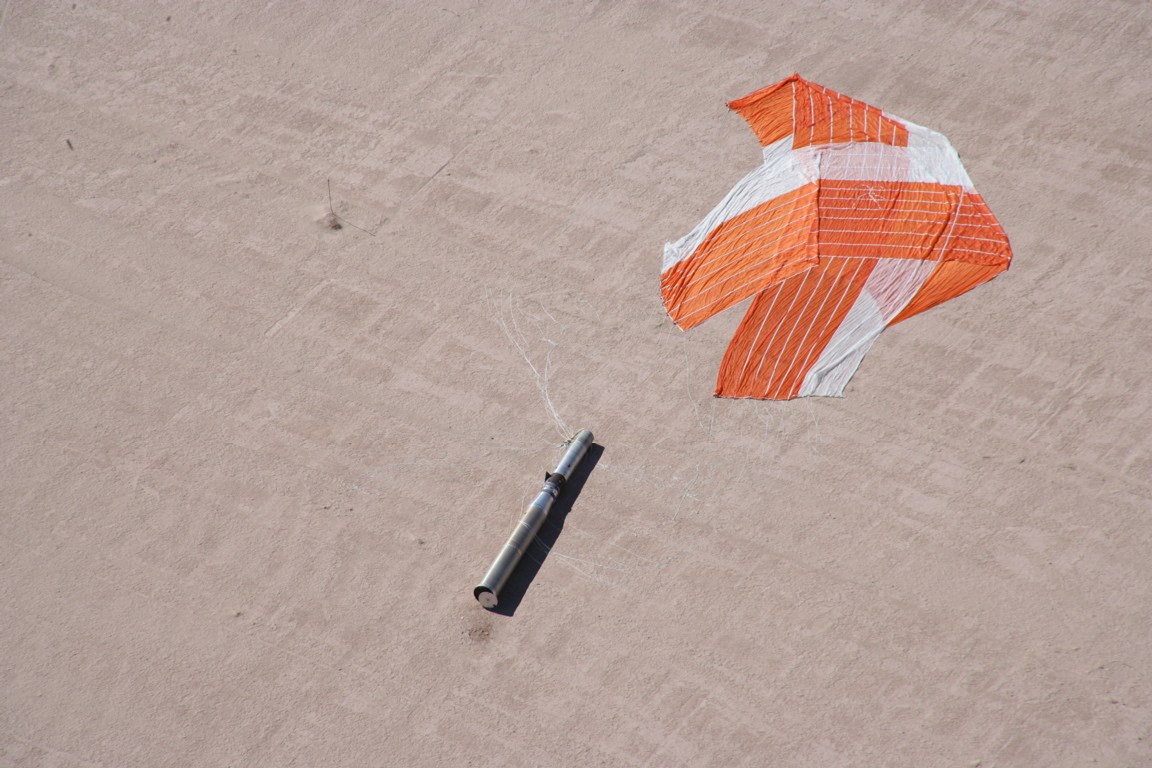
\includegraphics[width=0.9\textwidth]{images/desert}
				\caption{Synclink USB Adapter (above) and MOSES I after landing at WSMR (below)}
			\end{figure}
			
		\end{column}%
		\hfill%
		\begin{column}{.49\textwidth}

			\begin{itemize}
				\item Data is recovered off of SD card after landing.
				\item High-Speed Telemetry at 10 Mbit/s.
				\begin{itemize}
					\item Provided as backup in the event the payload is not recovered.
			  		\item 10.1 s per image.
			  		\item Each image takes $> \SI{5}{s}$.
			  	\end{itemize}				
				\item Synclink USB Adapter
				\begin{itemize}
					\item Transmitting and receiving units.
				\end{itemize}
				\item Groundstation Laptop
				\begin{itemize}
					\item receiveTM program with IDL image viewer.
				\end{itemize}
		  	\end{itemize}
					
		\end{column}%
		\end{columns}

	\end{frame}
	
	\begin{frame}
		
		\frametitle{Next Launch}
		
		\begin{columns}[T] % align columns
		\begin{column}{.49\textwidth}

			\begin{itemize}
				\item Scheduled for launch August 20th.
				\item Horizontal test
				\begin{itemize}
					\item Proving control and functionality over other payload components.
					\item Successful STIMS and dark exposure test confirms ROE functionality.
					\item Shutter and other subsystems have yet to be tested.
				\end{itemize}
				\item Flight model still needs to be completed.
				\item System must undergo thermal and vibrational testing.
			\end{itemize}			
			
		\end{column}%
		\hfill%
		\begin{column}{.49\textwidth}

			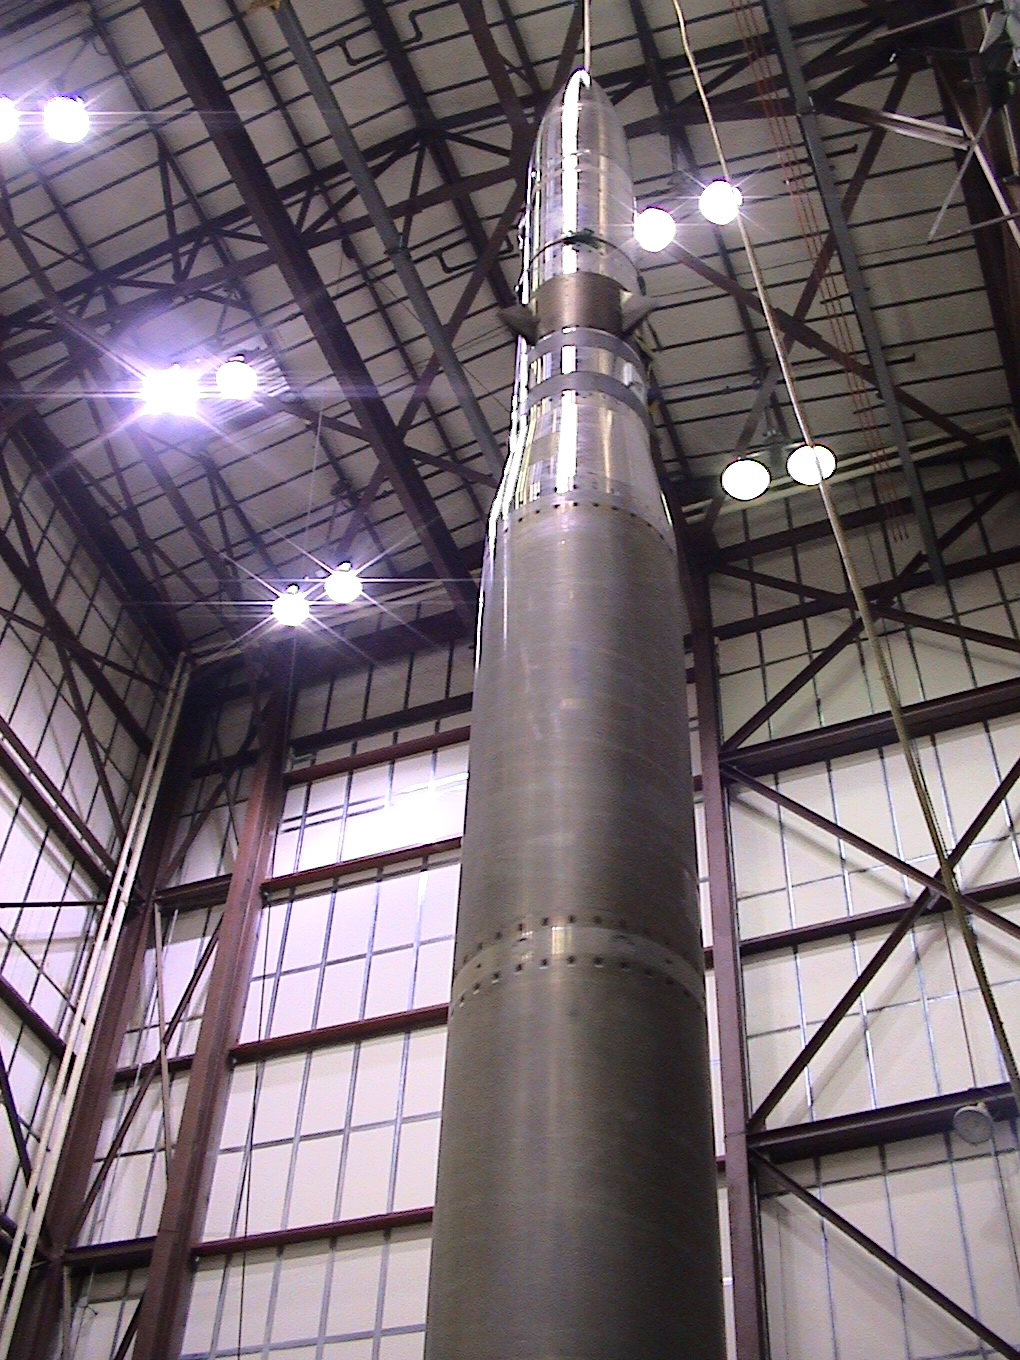
\includegraphics[width=\textwidth]{images/high}
					
		\end{column}%
		\end{columns}

	\end{frame}
	
	\begin{frame}
		\frametitle{References and Acknowledgements}
		
			This work is supported by NASA grant NNX14AK71G. \\[2cm]
		
		\bibliographystyle{unsrt}
		\bibliography{sources}
		
		
	\end{frame}
	
\end{document}








